%% LyX 1.3 created this file.  For more info, see http://www.lyx.org/.
%% Do not edit unless you really know what you are doing.
\documentclass[english, 12pt]{article}
\usepackage{times}
%\usepackage{algorithm2e}
\usepackage{url}
\usepackage{bbm}
\usepackage[T1]{fontenc}
\usepackage[latin1]{inputenc}
\usepackage{geometry}
\geometry{verbose,letterpaper,tmargin=2cm,bmargin=2cm,lmargin=1.5cm,rmargin=1.5cm}
\usepackage{rotating}
\usepackage{color}
\usepackage{graphicx}
\usepackage{amsmath, amsthm, amssymb}
\usepackage{setspace}
\usepackage{lineno}
\usepackage{hyperref}
\usepackage{bbm}
\usepackage{makecell}

\renewcommand{\arraystretch}{1.3}

\usepackage{xr}
\externaldocument{240pgs-supp}

%\linenumbers
%\doublespacing
\onehalfspacing
%\usepackage[authoryear]{natbib}
\usepackage{natbib} \bibpunct{(}{)}{;}{author-year}{}{,}

%Pour les rajouts
\usepackage{color}
\definecolor{trustcolor}{rgb}{0,0,1}

\def \NBTRAIT {240}

\usepackage{dsfont}
\usepackage[warn]{textcomp}
\usepackage{adjustbox}
\usepackage{multirow}
\usepackage{graphicx}
\graphicspath{{../figures/}}
\DeclareMathOperator*{\argmin}{\arg\!\min}
\usepackage{algorithm}
\usepackage{algpseudocode}

\let\tabbeg\tabular
\let\tabend\endtabular
\renewenvironment{tabular}{\begin{adjustbox}{max width=0.9\textwidth}\tabbeg}{\tabend\end{adjustbox}}

\makeatletter

%%%%%%%%%%%%%%%%%%%%%%%%%%%%%% LyX specific LaTeX commands.
%% Bold symbol macro for standard LaTeX users
%\newcommand{\boldsymbol}[1]{\mbox{\boldmath $#1$}}

%% Because html converters don't know tabularnewline
\providecommand{\tabularnewline}{\\}

\usepackage{babel}
\makeatother


\begin{document}


\title{Application Note:\\Optimal Linkage Disequilibrium Splitting}
\author{Florian Priv\'e$^{\text{1}}$}

\date{~ }
\maketitle

\noindent$^{\text{\sf 1}}$National Centre for Register-Based Research, Aarhus University, Aarhus, 8210, Denmark. \\

\noindent Contact: \url{florian.prive.21@gmail.com}

\vspace*{4em}

\abstract{
	A few algorithms have been developed for splitting the genome in nearly independent blocks of linkage disequilibrium.
	Due to the complexity of this problem, these algorithms rely on heuristics, which makes them sub-optimal.
	Here we develop an optimal solution for this problem using dynamic programming.
	This is now implemented as function \texttt{snp\_ldplit} as part of R package bigsnpr.
}

\clearpage



%%%%%%%%%%%%%%%%%%%%%%%%%%%%%%%%%%%%%%%%%%%%%%%%%%%%%%%%%%%%%%%%%%%%%%%%%%%%%%%%

\section*{Introduction}


\section*{Implementation}

We aim at optimally splitting the genome into $K$ blocks, where each block has a bounded number of variants (minimum and maximum).
This splitting is optimal in the sense that it minimizes the sum of squared correlations between blocks (hereinafter denoted as ``cost'').
This problem is quite complex, and a naive solution would be exponential with the number of variants.
To solve this problem efficiently, we use dynamic programming, which consists in breaking a problem into sub-problems and then recursively finding the optimal solutions to the sub-problems.
Each problem consists in solving
\begin{equation}
C(i, k) = \min_j \left(E(i, j) + C(j + 1, k - 1)\right) ~,
\end{equation}
where $C(i, k)$ is the minimum cost to split the region from variant $i$ to the last variant into $k$ blocks exactly, and $E(i, j)$ is the error that is added to the cost corresponding to defining variant $j$ as the last variant of the first block of this region. This is illustrated in figure \ref{fig:illu}.

\begin{figure}[h]
	\centering
	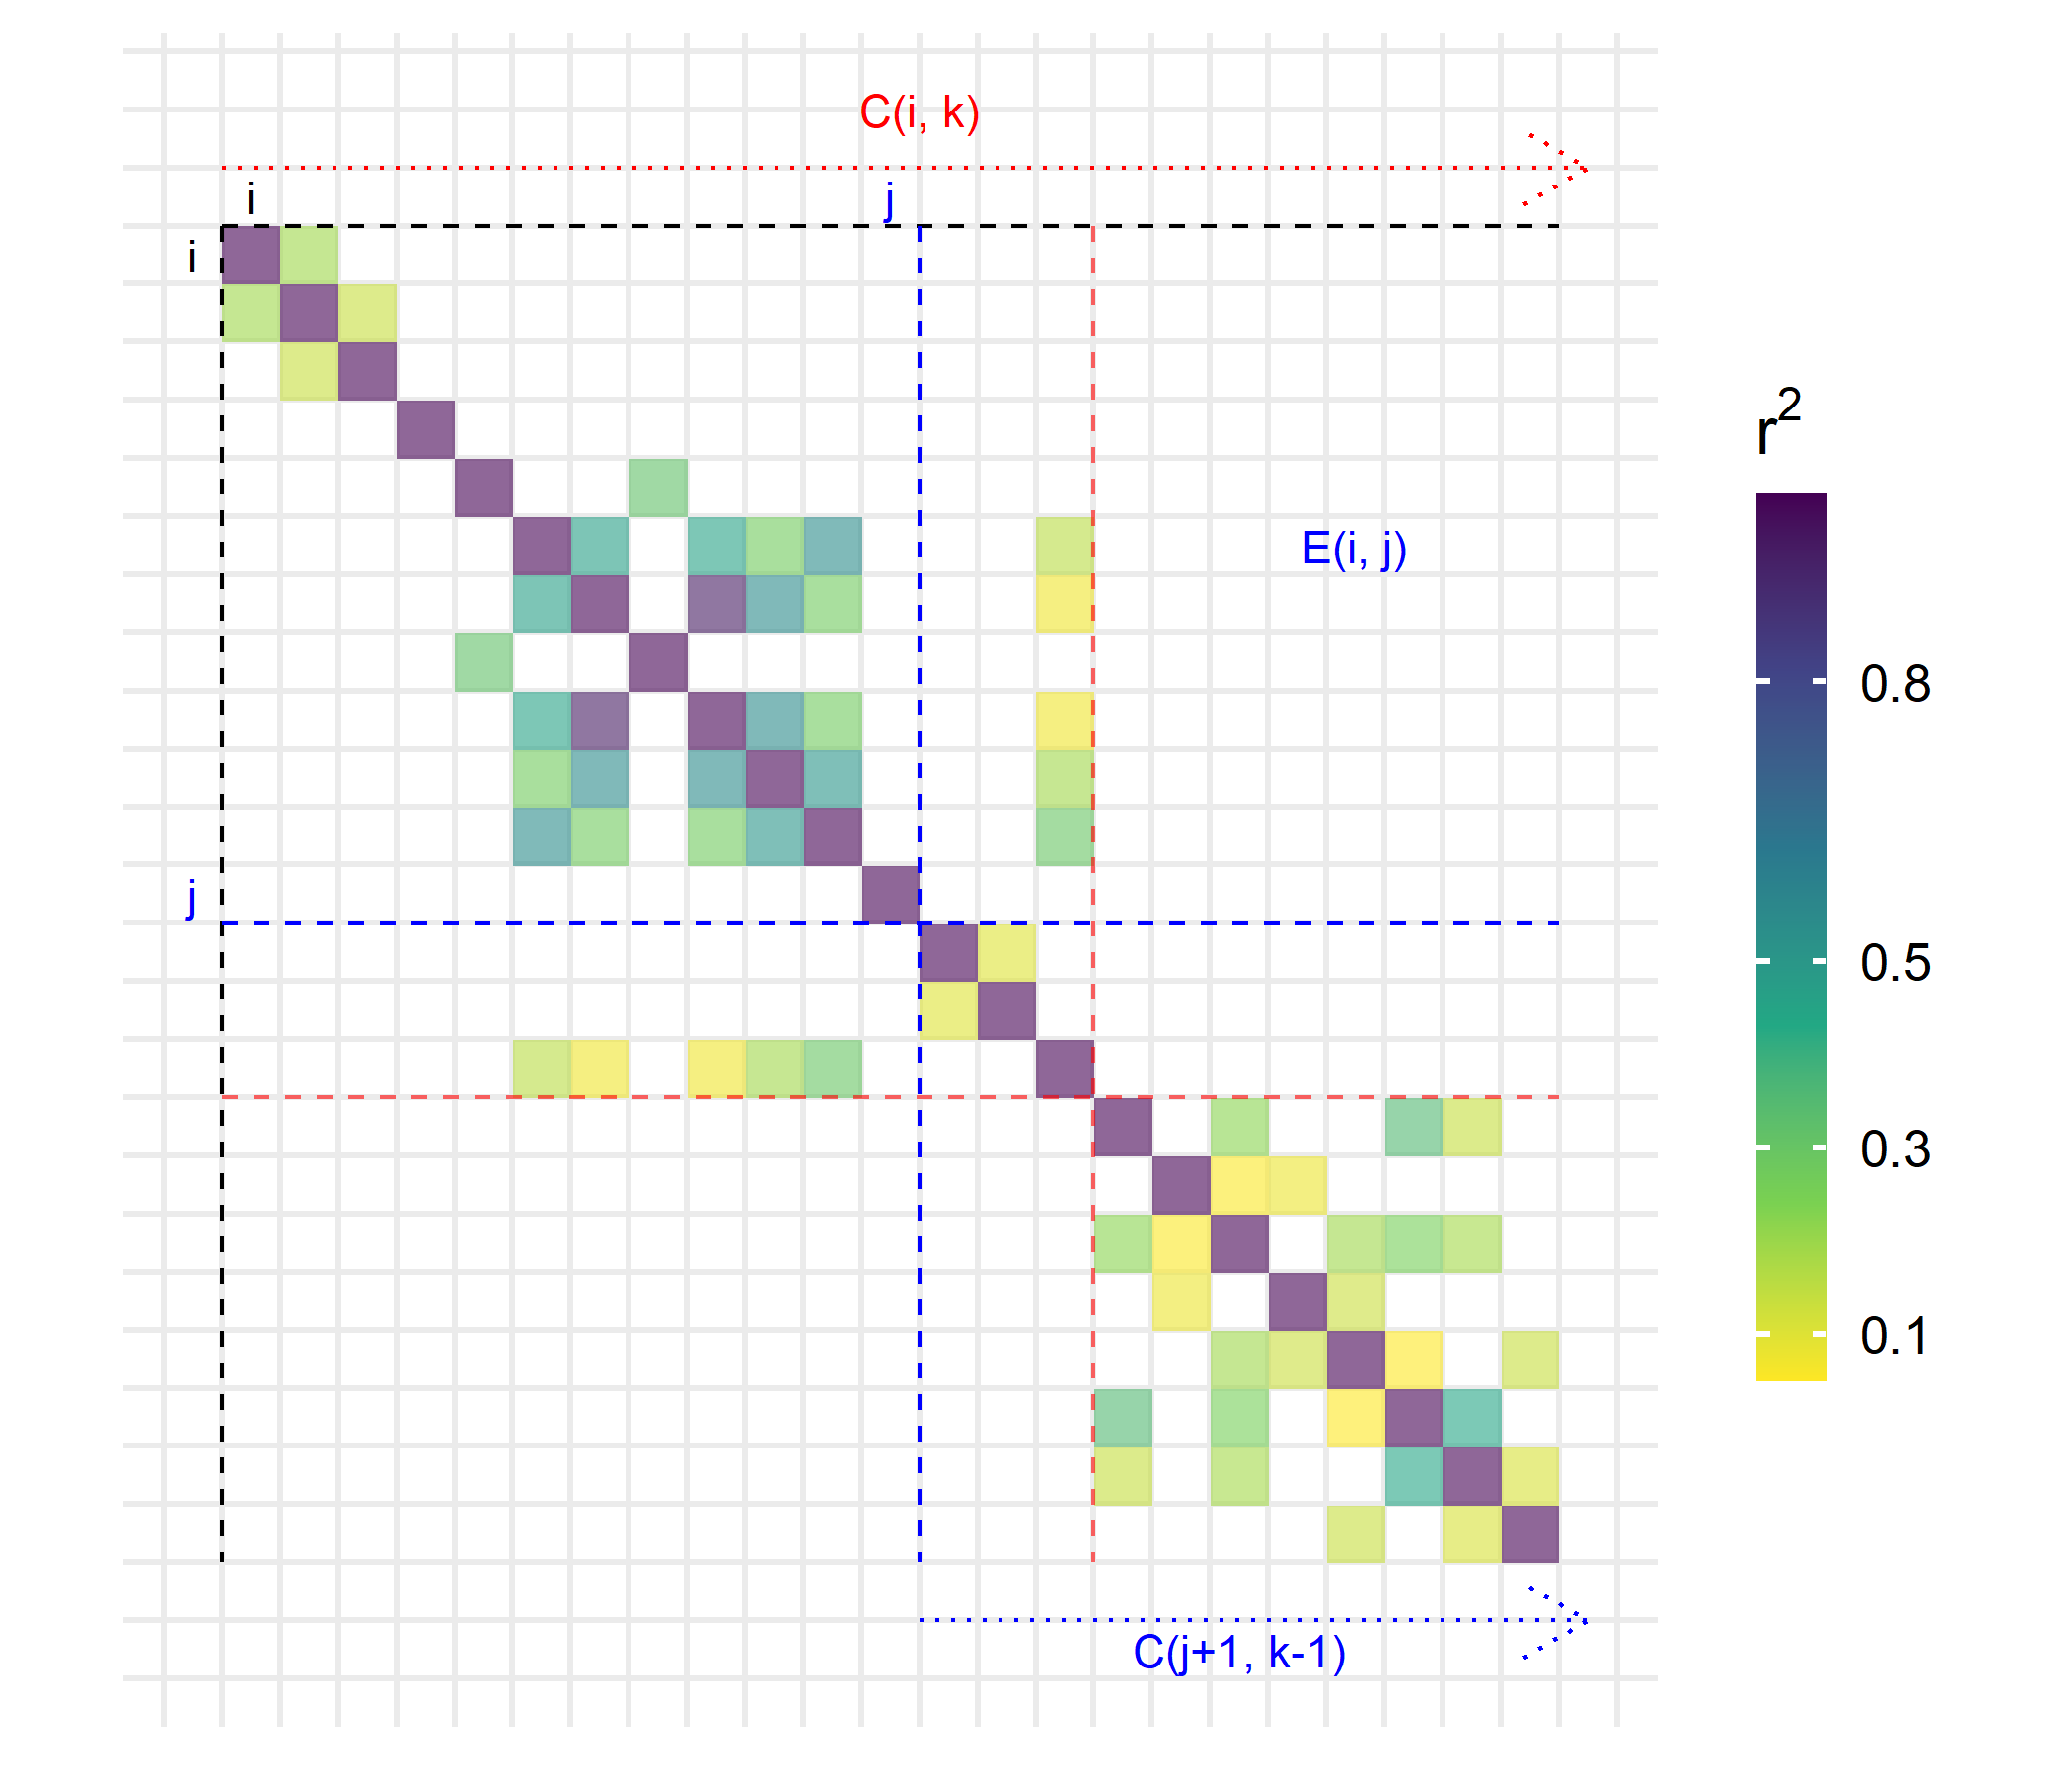
\includegraphics[width=0.8\textwidth]{illu}
	\caption{Illustration of sub-problems solved by the algorithm using a small LD matrix. The cost of separating the region starting at variant $i$ in $k$ blocks exactly, $C(i, k)$, is broken down in two: the error $E(i,j)$, the sum of all squared correlations between the block $(i,j)$ and all the later blocks, and the cost of separating the rest starting at $j+1$ using $(k-1)$ blocks. The variant $j$ at which the split occurs is chosen so that $\left(E(i, j) + C(j + 1, k - 1)\right)$ is minimized.}
	\label{fig:illu}
\end{figure}

These sub-problems can be solved efficiently by starting with $k=1$ and with $i$ from the end of the region.
Once all costs in the matrix $C$ have been computed, and corresponding splits $j$ have been recorded, the complete set of splits can be reconstructed from $C(1, K)$, where $K$ is the number of blocks desired.

\section*{Discussion}

DISCUSS ABOUT HYPER-PARAMETERS


%%%%%%%%%%%%%%%%%%%%%%%%%%%%%%%%%%%%%%%%%%%%%%%%%%%%%%%%%%%%%%%%%%%%%%%%%%%%%%%%

%\clearpage
%\vspace*{5em}

\section*{Software and code availability}

%All code used for this paper is available at \url{https://github.com/privefl/UKBB-PGS/tree/master/code}. 

\section*{Acknowledgements}

Authors thank GenomeDK and Aarhus University for providing computational resources and support that contributed to these research results.
This research has been conducted using the UK Biobank Resource under Application Number 58024.

\section*{Funding}

F.P. is supported by the Danish National Research Foundation (Niels Bohr Professorship to Prof. John McGrath).

\noindent\textit{Conflict of Interest:} none declared.

%%%%%%%%%%%%%%%%%%%%%%%%%%%%%%%%%%%%%%%%%%%%%%%%%%%%%%%%%%%%%%%%%%%%%%%%%%%%%%%%

\clearpage

\bibliographystyle{natbib}
\bibliography{refs}

%%%%%%%%%%%%%%%%%%%%%%%%%%%%%%%%%%%%%%%%%%%%%%%%%%%%%%%%%%%%%%%%%%%%%%%%%%%%%%%%


\end{document}
